% Figure: MHA / GQA / MQA / MLA as four rows sharing one frame -- how many K/V
% representations are cached per token, and the resulting cache size on one scale.
% Design width ~168mm, height ~66mm.
\documentclass[border=0pt]{standalone}
\usepackage{amsmath,amssymb}
% Shared visual language for the figures of the book.
% Every figure in this directory loads this file so the chapter reads as one system.
% NOTE: no blank lines are allowed inside \tikzset{...} (a blank line emits \par
% and breaks key scanning).
\NeedsTeXFormat{LaTeX2e}
\ProvidesPackage{figstyle}[2026/10/21 Figure style for Free Energy to LLMs]

\RequirePackage{tikz}
\usetikzlibrary{arrows.meta,positioning,calc,fit,shapes.geometric,shapes.misc,%
  backgrounds,matrix,decorations.pathreplacing,decorations.markings,patterns.meta}

% ---------------------------------------------------------------- palette
% Same values as book/preamble/style.tex, prefixed with F.
\definecolor{FNavy}{HTML}{14324A}
\definecolor{FTeal}{HTML}{0E7490}
\definecolor{FSky}{HTML}{E7F5F8}
\definecolor{FOrange}{HTML}{D97706}
\definecolor{FAmber}{HTML}{FFF3D6}
\definecolor{FInk}{HTML}{1F2937}
\definecolor{FSlate}{HTML}{64748B}
\definecolor{FMist}{HTML}{F5F7FA}
\definecolor{FRose}{HTML}{9F1239}
\definecolor{FRoseMist}{HTML}{FFF1F2}

% ---------------------------------------------------------------- semantics
% Teal   = probability / model / data object
% Orange = training objective, cost, or the quantity moved through the system
% Navy   = neutral structure
% Slate  = secondary label or metadata
% Rose   = failure mode, hazard, masked-out region
\tikzset{
  % Lay figures out in millimetres.  A figure designed 168mm wide is included at
  % \textwidth, so its fonts appear at exactly the size written here.
  every picture/.style={x=1mm,y=1mm,font=\small,line cap=round,line join=round},
  % ---- block styles
  nbase/.style={draw,rounded corners=1.2pt,align=center,inner sep=2.4pt,%
    minimum height=7mm,text=FInk},
  nteal/.style={nbase,draw=FTeal,fill=FSky},
  norange/.style={nbase,draw=FOrange,fill=FAmber},
  nnavy/.style={nbase,draw=FNavy,fill=white},
  nsoft/.style={nbase,draw=FSlate!55,fill=FMist},
  nrose/.style={nbase,draw=FRose,fill=FRoseMist},
  ghost/.style={draw=none,fill=none,align=center,inner sep=1pt},
  plain/.style={draw=none,fill=none,align=center,inner sep=0pt},
  % ---- arrows
  ar/.style={-{Latex[length=1.7mm,width=1.35mm]},draw=FSlate,line width=0.75pt},
  ard/.style={ar,dashed},
  arteal/.style={ar,draw=FTeal},
  arorange/.style={ar,draw=FOrange},
  arrose/.style={ar,draw=FRose},
  thickar/.style={ar,line width=1.2pt},
  % ---- text roles
  ftitle/.style={font=\large\bfseries,text=FNavy,align=center},
  ptitle/.style={font=\small\bfseries,text=FNavy,align=center},
  ptitleo/.style={font=\small\bfseries,text=FOrange,align=center},
  lbl/.style={font=\scriptsize,text=FSlate,align=center,inner sep=1pt},
  lblt/.style={lbl,text=FTeal},
  lblo/.style={lbl,text=FOrange},
  lbln/.style={lbl,text=FNavy},
  lblr/.style={lbl,text=FRose},
  sub/.style={font=\scriptsize,text=FSlate!90,align=center,inner sep=1pt},
  monob/.style={font=\ttfamily\scriptsize,text=FInk,inner sep=1pt},
  mathb/.style={font=\small,text=FInk,inner sep=1pt},
  eqn/.style={font=\scriptsize,inner sep=1.5pt,text=FInk},
  % ---- decorations
  brace/.style={decorate,decoration={brace,amplitude=2.4pt},draw=FSlate,%
    line width=0.6pt},
  bracet/.style={brace,draw=FTeal},
  braceo/.style={brace,draw=FOrange},
  axis/.style={draw=FSlate!55,line width=0.6pt},
  guide/.style={draw=FSlate!45,line width=0.5pt,dashed},
  halolabel/.style={font=\scriptsize,text=FInk,fill=white,fill opacity=0.85,%
    text opacity=1,inner sep=1.4pt,align=center},
}

% Figure title above the drawing, anchored at the figure's top-left.
\newcommand{\figtitle}[2][0]{%
  \node[ftitle,anchor=north west,outer sep=0pt] at (#1,0) {#2};}

% Rounded panel behind a subgroup of nodes.
\newcommand{\figpanel}[3][]{%
  \node[draw=FSlate!35,fill=#3,rounded corners=2pt,inner sep=2.6mm,#1] {#2};}

\endinput

\begin{document}
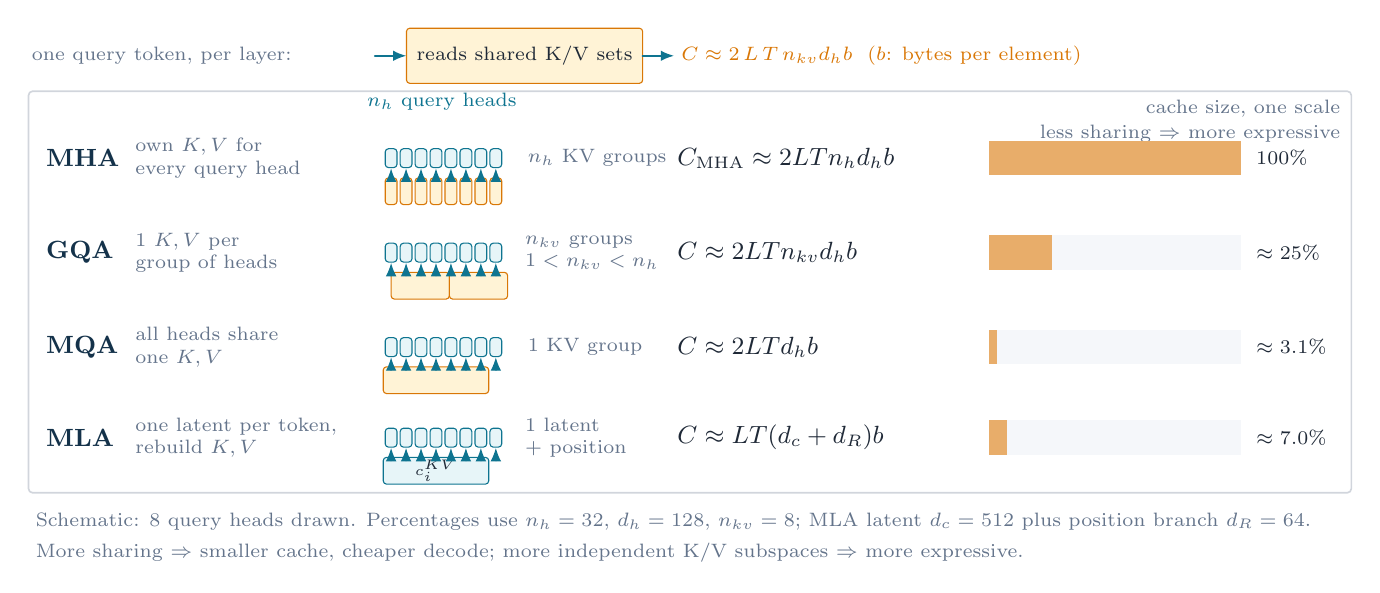
\begin{tikzpicture}
% ==================================================== top: what the cache is
\node[lbl,anchor=west] at (0,55) {one query token, per layer:};
\draw[arteal] (44,55)--(48,55);
\node[norange,minimum width=30mm,minimum height=7mm,font=\scriptsize,inner sep=1pt]
  (kvs) at (63,55) {reads shared K/V sets};
\draw[arteal] (78,55)--(82,55);
\node[lblo,anchor=west] at (82.5,55)
  {$C\approx 2\,L\,T\,n_{kv}d_h b$ \ ($b$: bytes per element)};

% ==================================================== four rows, one shared frame
\draw[FSlate!30,line width=0.6pt,rounded corners=1.5pt] (0,-0.5) rectangle (168,50.5);
\node[lblt,anchor=south,font=\scriptsize] at (52.5,47.6) {$n_h$ query heads};
\node[lbl,anchor=north east,align=right,font=\scriptsize] at (167,49.8)
  {cache size, one scale\\[1pt]
   less sharing $\Rightarrow$ more expressive};

\def\qpx{1.9}
\def\cz{52.7}
\def\barx{122}
\def\barw{32}

% ---------------------------------------------------------------- MHA
\def\ry{42}
\node[font=\small\bfseries,text=FNavy,anchor=west] at (1,\ry) {MHA};
\node[lbl,anchor=west,align=left,font=\scriptsize,inner sep=0pt] at (13.5,\ry)
  {own $K,V$ for\\every query head};
\foreach \i in {0,...,7}{
  \node[nteal,minimum width=1.5mm,minimum height=2.4mm,inner sep=0pt]
    (q\i) at ({46.05+\i*1.9},\ry) {};
  \node[norange,minimum width=1.5mm,minimum height=3.4mm,inner sep=0pt]
    (k\i) at ({46.05+\i*1.9},\ry-4.2) {};
  \draw[arteal,line width=0.5pt] ({46.05+\i*1.9},\ry-2.5)--({46.05+\i*1.9},\ry-1.3);}
\node[lbl,anchor=west,font=\scriptsize] at (63,\ry) {$n_h$ KV groups};
\node[mathb,anchor=west] at (82,\ry) {$C_{\mathrm{MHA}}\approx 2LTn_hd_hb$};
\fill[FMist] (122,39.8) rectangle (154,44.2);
\fill[FOrange!60] (122,39.8) rectangle (154,44.2);
\node[lbl,anchor=west,font=\scriptsize,text=FInk] at (155.5,\ry) {100\%};

% ---------------------------------------------------------------- GQA
\def\ry{30}
\node[font=\small\bfseries,text=FNavy,anchor=west] at (1,\ry) {GQA};
\node[lbl,anchor=west,align=left,font=\scriptsize,inner sep=0pt] at (13.5,\ry)
  {$1$ $K,V$ per\\group of heads};
\foreach \g in {0,1}{
  \node[norange,minimum width=7.4mm,minimum height=3.4mm,inner sep=0pt]
    at ({49.75+\g*7.4},\ry-4.2) {};}
\foreach \i in {0,...,7}{
  \node[nteal,minimum width=1.5mm,minimum height=2.4mm,inner sep=0pt]
    at ({46.05+\i*1.9},\ry) {};
  \draw[arteal,line width=0.5pt] ({46.05+\i*1.9},\ry-2.5)--({46.05+\i*1.9},\ry-1.3);}
\node[lbl,anchor=west,align=left,font=\scriptsize,inner sep=0pt] at (63,\ry)
  {$n_{kv}$ groups\\$1<n_{kv}<n_h$};
\node[mathb,anchor=west] at (82,\ry) {$C\approx 2LTn_{kv}d_hb$};
\fill[FMist] (122,27.8) rectangle (154,32.2);
\fill[FOrange!60] (122,27.8) rectangle (130,32.2);
\node[lbl,anchor=west,font=\scriptsize,text=FInk] at (155.5,\ry) {$\approx25\%$};

% ---------------------------------------------------------------- MQA
\def\ry{18}
\node[font=\small\bfseries,text=FNavy,anchor=west] at (1,\ry) {MQA};
\node[lbl,anchor=west,align=left,font=\scriptsize,inner sep=0pt] at (13.5,\ry)
  {all heads share\\one $K,V$};
\node[norange,minimum width=13.4mm,minimum height=3.4mm,inner sep=0pt]
  at (51.75,\ry-4.2) {};
\foreach \i in {0,...,7}{
  \node[nteal,minimum width=1.5mm,minimum height=2.4mm,inner sep=0pt]
    at ({46.05+\i*1.9},\ry) {};
  \draw[arteal,line width=0.5pt] ({46.05+\i*1.9},\ry-2.5)--({46.05+\i*1.9},\ry-1.3);}
\node[lbl,anchor=west,font=\scriptsize] at (63,\ry) {$1$ KV group};
\node[mathb,anchor=west] at (82,\ry) {$C\approx 2LTd_hb$};
\fill[FMist] (122,15.8) rectangle (154,20.2);
\fill[FOrange!60] (122,15.8) rectangle (123,20.2);
\node[lbl,anchor=west,font=\scriptsize,text=FInk] at (155.5,\ry) {$\approx3.1\%$};

% ---------------------------------------------------------------- MLA
\def\ry{6.5}
\node[font=\small\bfseries,text=FNavy,anchor=west] at (1,\ry) {MLA};
\node[lbl,anchor=west,align=left,font=\scriptsize,inner sep=0pt] at (13.5,\ry)
  {one latent per token,\\rebuild $K,V$};
\node[nteal,minimum width=13.4mm,minimum height=3.4mm,inner sep=0pt,font=\tiny]
  at (51.75,\ry-4.2) {$c_i^{KV}$};
\foreach \i in {0,...,7}{
  \node[nteal,minimum width=1.5mm,minimum height=2.4mm,inner sep=0pt]
    at ({46.05+\i*1.9},\ry) {};
  \draw[arteal,line width=0.5pt] ({46.05+\i*1.9},\ry-2.5)--({46.05+\i*1.9},\ry-1.3);}
\node[lbl,anchor=west,align=left,font=\scriptsize,inner sep=0pt] at (63,\ry)
  {$1$ latent\\$+$ position};
\node[mathb,anchor=west] at (82,\ry) {$C\approx LT(d_c+d_R)b$};
\fill[FMist] (122,4.3) rectangle (154,8.7);
\fill[FOrange!60] (122,4.3) rectangle (124.25,8.7);
\node[lbl,anchor=west,font=\scriptsize,text=FInk] at (155.5,\ry) {$\approx7.0\%$};

% ---------------------------------------------------------------- notes
\node[lbl,anchor=north west,align=left,font=\scriptsize] at (0.5,-2.6)
  {Schematic: 8 query heads drawn. Percentages use $n_h=32$, $d_h=128$, $n_{kv}=8$;
   MLA latent $d_c=512$ plus position branch $d_R=64$.};
\node[lbl,anchor=north west,align=left,font=\scriptsize] at (0.5,-6.4)
  {More sharing $\Rightarrow$ smaller cache, cheaper decode;
   more independent K/V subspaces $\Rightarrow$ more expressive.};
\end{tikzpicture}
\end{document}
